\section{Results}\label{sec:results}

\subsection{Engine speed}
Figure~\ref{fig:speed} compares stock and snapshot cg14 on the six models: fdtdKit at each model's best thread count,
stock at its best for the four tutorial models and at 4 threads for the two boards, whose stock thread count was not
swept. Figure~\ref{fig:progress} shows how the speed-up accumulated snapshot by snapshot (Table~\ref{tab:snapshots}
names them); Figure~\ref{fig:threads} and Table~\ref{tab:final} give the thread scaling of cg14 and the automatic
choice. These engine-speed figures and tables stop at cg14. Snapshot cg18 (patches 0001--0006, the build installed on
the author's Mac from 2026-11-04 to 2026-11-06) went through the same full check on a quiet machine on 2026-11-03
(\code{results/*\_cg18.txt}):
bit-identical to stock on all six
models; its best speeds differ from cg14's by $-2.7$ to $+1.6$\,\% on five models and by $+8.2$\,\% on the GCPW line
(whose cg13 run had reached 1\,745\,\MC); on the four models of up to about a million cells it reaches
1\,361--1\,961\,\MC, 3.1--6.8$\times$ the stock rows of the same tables. The cg17 tables in \code{results/} are
correctness checks, run while the machine was loaded. The current build, cg29, is compared with stock on the CPU and
on the Metal diamond engine in Section~\ref{sec:current}.

Part of the patch tutorial's factor is not the patches' (\code{results/*\_base.txt}, 2026-11-03, best of two runs on
a quiet machine). The fork's base, upstream's \code{gpu-engine} branch at 7bb294f with stock's CSXCAD and nf2ff
libraries, runs that model 1.13$\times$ faster than stock (308.5 against 273.4\,\MC, both at their best, 2 threads),
all of it on the dump side: with the dumps off both reach 342.2\,\MC\ at 2 threads. The difference is the base's
background HDF5 writer, which writes the model's 12 time-domain dumps off the main thread and keeps their files open
(the CPU engines still evaluate the dumps on the main thread; only the base's GPU engine evaluates them from a field
snapshot, and the Metal diamond engine of Section~\ref{sec:gpu} leaves them to the CPU between its calls). Snapshot
cg18 runs that model 5.98$\times$ faster than the base (1\,845.9\,\MC\ at 4 threads), so the
patches' own factor there is about 6.0$\times$. On the notch tutorial, the GCPW line and patch x5 the base runs within
0.98--1.03$\times$ of stock; the SMA launch was not run with it. Every run in these files has stock's probes and
$S$-parameters.

\begin{figure}[htbp]\centering
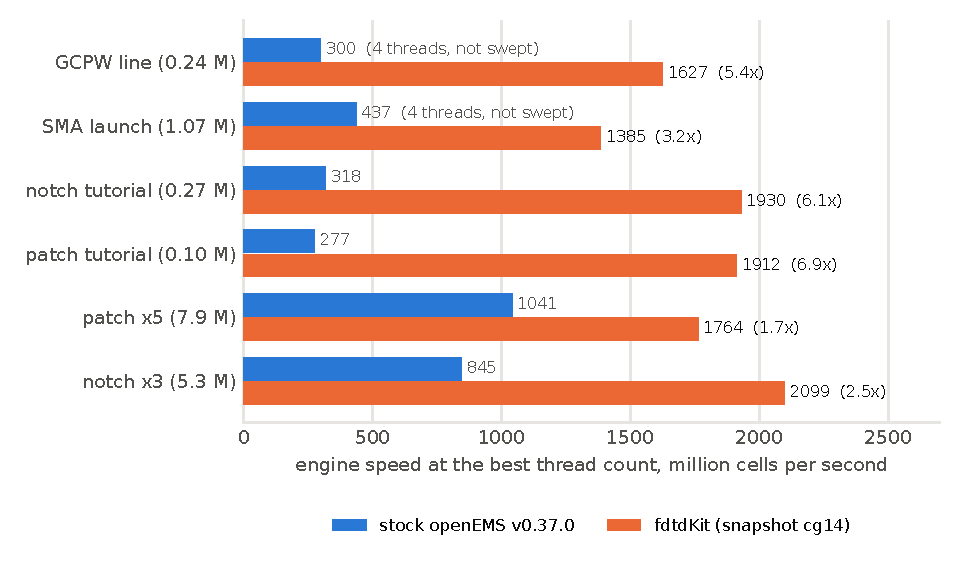
\includegraphics[width=0.9\textwidth]{fig_speed}
\caption{Stock v0.37.0 against fdtdKit snapshot cg14 (\code{results/*\_cg14.txt}), same results bit for bit. fdtdKit at
each model's best thread count; stock at its best for the tutorial models (Table~\ref{tab:step1}) and, for the two
boards, one 4-thread reference run each (the cg10 run for the GCPW line, the cg14 run for the SMA launch), as their
stock thread count was not swept. On the patch tutorial about 1.13$\times$ of the factor comes from the fork's base
(see the text).}\label{fig:speed}
\end{figure}

\begin{table}[p]\centering\footnotesize
\begin{tabular}{@{}lp{0.82\textwidth}@{}}
\toprule
snapshot & added \\
\midrule
A & spin barriers, hook plan \\
AB & + inner loop (IJKN) \\
ABCDEG & + work stealing, automatic thread count (0.15\,s windows), Mur fast path, UPML on vectors, fused sweep with
line hooks for Mur, UPML, excitation and lumped RLC, background HDF5 writer \\
cg, cg2 & rebased on upstream's gpu-engine branch at commit 7bb294f (its gather and asynchronous dumps; the branch has
since been deleted upstream), slab balancing; Field\_Gather\_SSE \\
cg6 & Mur line hooks vectorised in memory order (from cg4; the dump experiments of cg3 and cg5 removed) \\
cg8 & thread tuner timed in pieces of window/8 with slab balancing between them (cg7), refined search \\
cg9 & threaded operator setup, nf2ff matrix product, CSXCAD lookups, operator/field export \\
cg10 & staggered allocations (allocation-placement valley), \code{--disable-dumps} crash fix \\
cg11 & scalar-SSE UPML path for z-only PML slabs \\
cg12 & line hooks for the dispersive extensions (conducting sheets) \\
cg13 & packed coefficient tables \\
cg14 & compressed UPML coefficient tables \\
cg15 & user-initiated thread QoS \\
cg16 & probe end criterion \\
cg17 & review fixes (patch 0005): Debye hooks, probe end arming, setup cache key, portability guards
(Section~\ref{sec:reviewfixes}) \\
cg18 & final-review fixes (patch 0006): probe end with excitation delays and waveguide probes, packed tables always
built, on/off switches, tuner clamp, flush-to-zero state restored, size limits (Section~\ref{sec:reviewfixes}) \\
cg19 & Metal diamond engine, \code{--engine=metal-diamond} (0007): cell updates, excitation and Mur on the GPU
(Section~\ref{sec:gpu}) \\
cg20 & + lumped RLC elements on the GPU (0008) \\
cg21 & + UPML on the GPU; extension data in three buffers; threads per tile from the tile size (0009) \\
cg22 & + Drude/Lorentz materials and conducting sheets on the GPU: all six models run there (0010) \\
cg23 & + Debye materials on the GPU (0011) \\
cg24 & GPU engine's operator setup on all cores (\code{Operator\_Multithread}); \code{OPENEMS\_DIAMOND\_TIMING} (0012) \\
cg25 & excitation and dispersive elements as runs; per-tile offsets read once (0013) \\
cg26 & grid sizes as constants of the kernel; Mur and UPML records passed by value (0014) \\
cg27 & split coefficient tables for graded meshes (0015) \\
cg28 & tiling chosen at run time (0016) \\
cg29 & CPU items (0017--0027, one per topic; Section~\ref{sec:cg29}): operator index per z-vector, merged ADE for
conducting sheets, UPML y-rows, UPML setup on the setup threads (PR \#244), line hooks for the steady-state detection
and for Debye materials, geometry coefficient tables, \code{OPENEMS\_FUSED\_STAT}, neighbour flags instead of the two
barriers with RLC slots by time step (Discussion \#492), steady-state detection on the flags, no flag spin above the
P-core count \\
\bottomrule
\end{tabular}
\caption{Snapshots. Each is a complete set of dylibs plus the cumulative patch, kept for bisection on the author's
machine. \code{patches/openems/} publishes the fork as patches 0001--0027: 0001--0006 end at cg18 (0001 = cg8, 0002 =
cg9, 0003 = cg10--cg15, 0004 = cg16, 0005 = cg17, 0006 = cg18), the build installed on the author's Mac from
2026-11-04 to 2026-11-06; 0007--0016 are cg19--cg28, one per snapshot (Table~\ref{tab:gpucov}); 0017--0027 are cg29,
one per topic (Table~\ref{tab:cg29}), the build installed there since 2026-11-06. A row lists what the snapshot added
over the row above; the intermediate snapshots cg3--cg5 and cg7 appear inside the cg6 and cg8
rows.}\label{tab:snapshots}
\end{table}

\begin{figure}[htbp]\centering
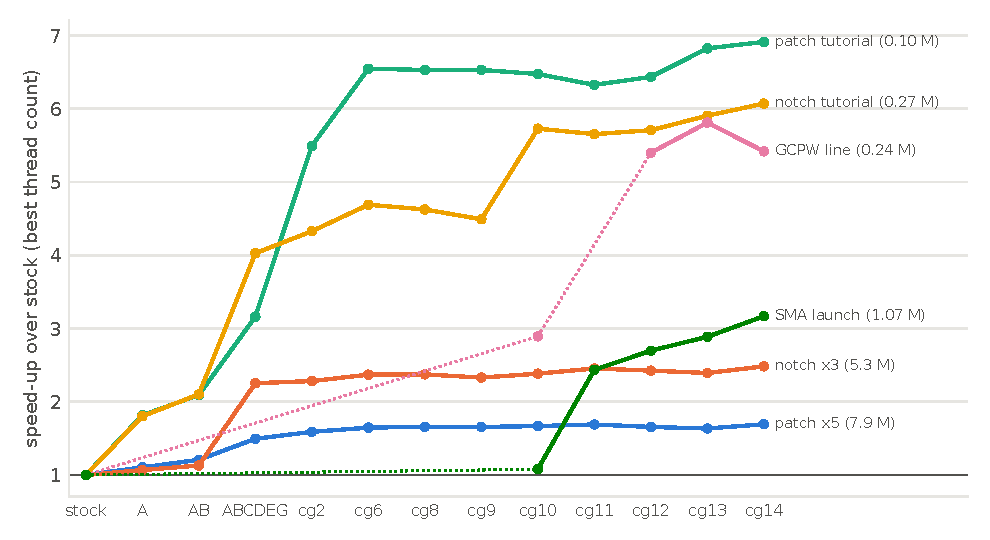
\includegraphics[width=0.95\textwidth]{fig_progress}
\caption{Speed-up over stock per snapshot (the best thread count of each check run; \code{results/summary.json}, which
\code{paper/figures/parse\_results.py} collects from the tables in \code{results/}). Stock as in
Figure~\ref{fig:speed}. The two boards joined the suite at cg10 and the GCPW line was not run at cg11; dotted lines
bridge those gaps. The two runs behind each value differ by 1.2\,\% in the median and by 9\,\% or more in one pair in
ten (399 pairs in the tables of 2026-10-28 and 2026-10-29 in \code{results/}), so steps of that size are noise: the
GCPW's from cg13 to cg14 (1\,745 to 1\,627\,\MC\ at 4 threads; the two cg13 runs gave 1\,745 and 1\,608) is one. The
patch x5 point of A (1\,151\,\MC, 8 threads) is a run whose load figure is invalid in its table; load can only slow a
run, so it is kept.}\label{fig:progress}
\end{figure}

\begin{figure}[htbp]\centering
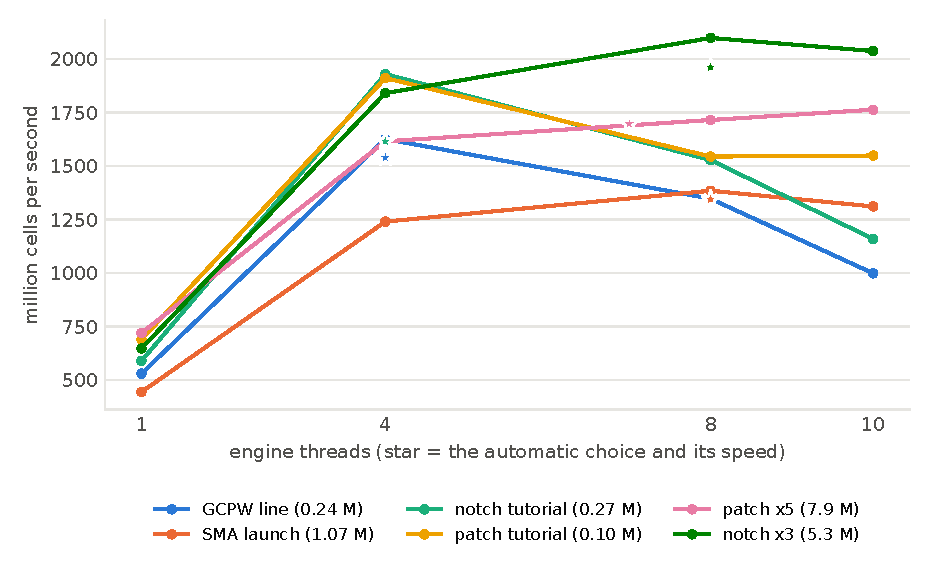
\includegraphics[width=0.85\textwidth]{fig_threads}
\caption{Thread scaling of snapshot cg14 (the check runs of 2026-10-29, \code{results/*\_cg14.txt}). Stars: the
automatic choice and the speed it reached, which includes the search of about 1.5\,s (project log; none for the patch
tutorial: its 0.7\,s run ends before the search prints its choice).}\label{fig:threads}
\end{figure}

\begin{table}[H]\centering\small
\begin{tabular}{@{}lrrrrrr@{}}
\toprule
model & stock (thr) & 1 thr & 4 thr & 8 thr & 10 thr & auto (picked) \\
\midrule
GCPW line (0.24\,M)      & 300 (4)  & 530 & 1627 & 1348 & 999  & 1540 (4) \\
SMA launch (1.07\,M)     & 437 (4)  & 444 & 1241 & 1385 & 1311 & 1344 (8) \\
notch tutorial (0.27\,M) & 318 (4)  & 590 & 1930 & 1528 & 1160 & 1615 (4) \\
patch tutorial (0.10\,M) & 277 (2)  & 690 & 1912 & 1545 & 1550 & 1499 (--) \\
patch x5 (7.9\,M)        & 1041 (8) & 720 & 1616 & 1716 & 1764 & 1697 (7) \\
notch x3 (5.3\,M)        & 845 (8)  & 648 & 1841 & 2099 & 2038 & 1962 (8) \\
\bottomrule
\end{tabular}
\caption{Snapshot cg14, \MC; fdtdKit columns from \code{results/*\_cg14.txt} (the run label in those files is
\code{cgy}). Stock: the best of the Table~\ref{tab:step1} sweep for the tutorials; for the two boards one 4-thread
reference run each (cg10 GCPW, cg14 SMA), as their stock thread count was not swept. The patch tutorial's 0.7\,s auto
run ends before the search prints its choice.}
\label{tab:final}
\end{table}

Two patterns of cg14 deserve a sentence. Single-thread speed rose 1.8 to 4.4 times over stock's sse-compressed engine
on the four models that have a stock single-thread run (Table~\ref{tab:step1}; the inner loop, the allocation
stagger, the boundary paths); of the patch tutorial's 2.7 times, the fork's base alone gives 1.18 times at one thread (296.6
against 251.3\,\MC, both with the multithreaded engine on one thread; \code{results/patch\_s1\_n10500\_base.txt}). And
the best thread count is 4 for models up to a few hundred thousand cells, where the four P cores saturate what the
per-step synchronisation leaves, and 8 to 10 above a million, where the E cores add bandwidth; the automatic choice
finds this within 3--7\,\% on the two boards and the two large models, while on the 0.6--2.7\,s tutorial runs the
search itself costs 16--22\,\% (in the cg18 check the GCPW line's 2.4\,s automatic run also lost 13\,\%). In cg29,
whose neighbour flags replace the two barriers per time step (Section~\ref{sec:cg29}), 8 threads was the fastest
setting measured on all six models, the smallest included (Section~\ref{sec:current}).

\subsection{The current build on the CPU and on the GPU (cg29)}\label{sec:current}
Table~\ref{tab:current} sets the current build, cg29 (patches 0001--0027), against stock v0.37.0 on the six models,
on the CPU and on the Metal diamond engine of Section~\ref{sec:gpu}, in one paired interleaved run per model on
2026-11-05 (\code{results/speed\_cg29\_2026-11-05.txt}; 4 rounds, the step counts of \code{bench/check.sh}). On the
CPU, cg29's best setting of the three measured (4 and 8 threads and the automatic count) is 8 threads on every
model, the patch tutorial's 0.104\,M cells included; the automatic count ran 1.2--7.5\,\% below it (the medians of
the rows). At 8 threads cg29 runs the four models of up to about a million cells at 1\,808--1\,961\,\MC,
4.73--6.89$\times$ stock at stock's best of 2, 4 and 8 threads, and the two large models at 1\,958 (patch x5) and
2\,177\,\MC\ (notch x3), 1.95$\times$ and 2.72$\times$. The Metal diamond engine runs the four at 4.83--7.40$\times$
stock and the two large models at 2.87$\times$ and 3.99$\times$. Against the CPU engine at its best, paired in the
same rounds, it is ahead on patch x5 (1.47$\times$), notch x3 (1.46$\times$) and the GCPW line (1.17$\times$), level
on the SMA launch (1.00$\times$; 0.99--1.13 over the rounds) and behind on the notch tutorial (0.97$\times$) and the
patch tutorial (0.93$\times$). Grid size decides most of this (Figure~\ref{fig:crossover}): in a sweep of three models
over 0.1--7.9\,M cells the GPU led in every round from 1.7--2.9\,M cells on and by 1.25--1.52$\times$ above 3\,M, and
below that the two engines were within 0.89--1.23$\times$ of each other, the side depending on the model and on the
session. On the patch tutorial, whose nf2ff dumps end a GPU call every 31 steps, the GPU stands idle for 18--27\,\% of the
time-stepping loop, while the CPU evaluates the dumps and while each call's command buffers start and finish; on the
notch tutorial it is busy 97\,\% of the time but runs slower on so small a grid
(Section~\ref{sec:gpu}).

Every CPU run's port probes are identical to stock's at 4 threads. The GPU runs differ from them by
$1.7\times10^{-7}$ to $9.4\times10^{-7}$ relative: Apple's GPU flushes subnormal numbers to zero and the CPU keeps
them, and with \code{OPENEMS\_FTZ=1} on the CPU the two engines are identical on all six models
(\code{results/*\_cg29gpu.txt}; Section~\ref{sec:policy}). The SMA launch runs here on the 1.071\,M-cell mesh of the
earlier tables (\code{RFSIM\_MIN\_CELL=0.02}), not on the 0.871\,M cells that the toolkit's default has built since
2026-11-04 (Table~\ref{tab:models}); rates on the two meshes do not compare. A round started once the other processes
were quiet and was run again (on the SMA launch, a single run) when they rose above the limit during it (the caption
gives the rule); during the runs kept the others used a median of 0.5--0.8 cores per model, at most 1.5.

Two things set Table~\ref{tab:current} apart from Table~\ref{tab:final}: its stock reference ran in the same rounds,
at 2, 4 and 8 threads on every model, while Table~\ref{tab:final} took stock's rates for the tutorials from the
step-1 sweep and one 4-thread run for each board; and its snapshot is cg29, not cg14. Stock's rates also differ
between the two sessions (the SMA launch at 4 threads 437 against 379\,\MC, both on the 1.071\,M mesh), so the ratio
of the two tables' factors is not cg29's gain over cg14. For cg29 against cg18, paired with each other in rounds of
their own over the six models (5 rounds, other processes on 0.3--0.6 cores, the SMA launch on its 0.871\,M mesh),
Section~\ref{sec:cg29} gives 1.03--1.23$\times$ at 4 threads and 1.13--1.44$\times$ at 8
(\code{results/cpu\_items\_cg29\_2026-11-05.txt}, section 4).

% Generated by figures/tables.py from results/speed_cg29_2026-11-05.txt; edit the script, not this file.
\begin{table}[H]\centering\small
\resizebox{\ifdim\width>\textwidth\textwidth\else\width\fi}{!}{\begin{tabular}{@{}lrrrrrrrr@{}}
\toprule
 & stock v0.37.0 & \multicolumn{3}{c}{cg29, CPU (multithreaded)} & cg29, GPU & \multicolumn{3}{c@{}}{paired ratio} \\
\cmidrule(lr){2-2}\cmidrule(lr){3-5}\cmidrule(lr){6-6}\cmidrule(l){7-9}
model (cells) & best (thr) & 4 thr & 8 thr & auto & diamond & CPU / stock & GPU / stock & GPU / CPU \\
\midrule
GCPW line (0.242\,M) & 286 (4) & 1548 & \textbf{1808} & 1689 & 2113 & 6.33 & 7.40 & 1.17 \\
SMA launch (1.071\,M) & 379 (4) & 1388 & \textbf{1833} & 1799 & 1829 & 4.73 & 4.83 & 1.00 \\
notch tutorial (0.270\,M) & 303 (4) & 1595 & \textbf{1961} & 1814 & 1893 & 6.56 & 6.26 & 0.97 \\
patch tutorial (0.104\,M) & 268 (2) & 1829 & \textbf{1854} & 1832 & 1729 & 6.89 & 6.48 & 0.93 \\
patch x5 (7.86\,M) & 1003 (8) & 1705 & \textbf{1958} & 1889 & 2879 & 1.95 & 2.87 & 1.47 \\
notch x3 (5.25\,M) & 800 (8) & 1736 & \textbf{2177} & 2097 & 3193 & 2.72 & 3.99 & 1.46 \\
\bottomrule
\end{tabular}}
\caption{Snapshot cg29 (patches 0001--0027) against stock v0.37.0 on the six models, \MC, measured on 2026-11-05 (\code{results/speed\_cg29\_2026-11-05.txt}). One paired interleaved run per model (\code{bench/abtest.py}, 4 rounds, the step counts of \code{bench/check.sh}): every round runs stock at 2, 4 and 8 threads, cg29's multithreaded engine at 4 and 8 threads and with the automatic thread count, and cg29's Metal diamond engine, in turn, once the other processes use at most 1.5 cores and 10\,\% of the GPU, and is run again, up to three times, when they rose above that during one of its runs; the SMA launch row comes from a re-run that repeats the single loaded runs instead (\code{--run-redo 3}). Rates: the median over the rounds; ratios: the median of the per-round ratios. Stock: the best of its three thread counts. Bold: cg29's best CPU setting, which the two CPU ratios use. Every CPU run's port probes are identical to stock's at 4 threads; the GPU runs differ from them by at most $9.4\times10^{-7}$ relative, because the GPU flushes subnormal numbers (with \code{OPENEMS\_FTZ=1} on the CPU they are identical, \code{results/*\_cg29gpu.txt}). The SMA launch on the 1.071\,M-cell mesh of the earlier tables (\code{RFSIM\_MIN\_CELL=0.02}); the toolkit's default since 2026-11-04 builds 0.871\,M cells. The other processes used a median of 0.5--0.8 cores per model during the runs kept.}\label{tab:current}
\end{table}


\subsection{End-to-end run time}
Figure~\ref{fig:runtime} and Table~\ref{tab:e2e} give the number the author cares about: the wall time of a complete
simulation of each board from the toolkit, timed around its \code{FDTD.Run} call (operator setup and time stepping).
All runs were made on 2026-11-03 with the toolkit as it was that day and the meshes it built, one per board with
stock v0.37.0 and one per setting with cg18 (\code{results/rfsim\_e2e\_2026-11-03.txt}). The columns are:
the full run with stock, which goes to \code{max\_time} because the energy criterion never fires
(Section~\ref{sec:probeend}); the same full run with fdtdKit, same steps, so the difference is the solver's alone;
fdtdKit with the probe end at $-60$\,dB and a hold of 1, the toolkit's default until 2026-11-04; and a hold of 0.5
with, on the SMA launch, the 0.05\,mm mesh floor of
Section~\ref{sec:meshfloor}, the shortest setting tested, which the author made the toolkit's default on 2026-11-04
(toolkit commit 4a7e20e). Model and Gaussian pulse are
the same in every column (the SMA launch's mesh is coarser in the last). The solver alone gives 5.6$\times$ on the
GCPW line and 3.3$\times$ on the SMA launch; the probe end with the earlier defaults brings this to 8.9$\times$ and
5.8$\times$, the toolkit's current defaults to 14.7$\times$ and 15.0$\times$, at the accuracy costs of
Tables~\ref{tab:probeend} and~\ref{tab:mesh}. Stock ran with the thread counts the toolkit uses
for a stock library, 4 on the GCPW line and 8 on the SMA launch, the same counts the tuner picked for the two full
runs. On the SMA launch this 8-thread stock run reached 348\,\MC, while stock's 4-thread bench run on the same board
reached 437\,\MC\ (Table~\ref{tab:final}): the SMA factors are against the toolkit's stock setting.

\begin{figure}[htbp]\centering
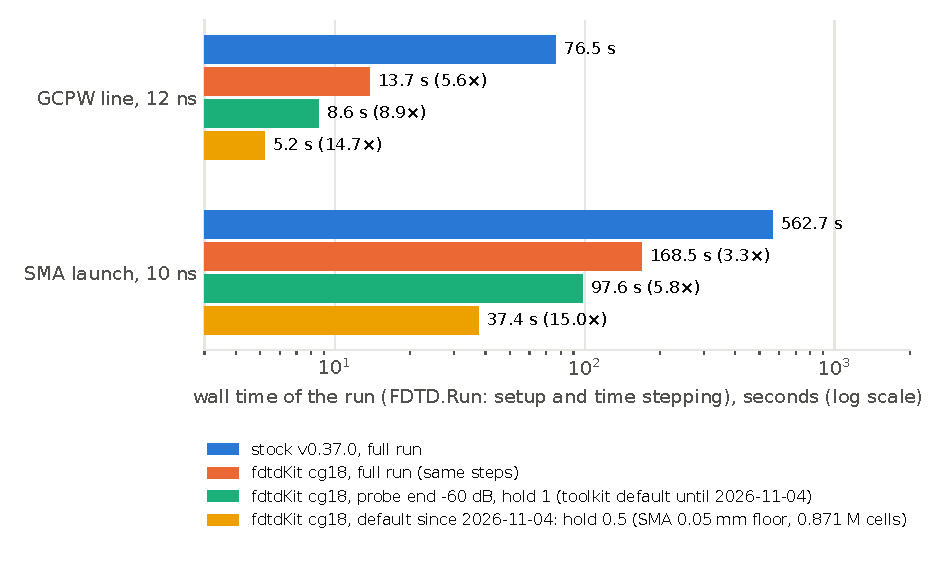
\includegraphics[width=0.85\textwidth]{fig_runtime}
\caption{Wall time of \code{FDTD.Run} for a complete simulation of the two boards, measured on 2026-11-03
(Table~\ref{tab:e2e}): stock v0.37.0 and fdtdKit (snapshot cg18) for the full run, cg18 with the probe end at
$-60$\,dB and a hold of 1 (the toolkit's default until 2026-11-04), and
cg18 with the toolkit's defaults since 2026-11-04 (a hold of 0.5; on the SMA launch also the 0.05\,mm mesh floor).
Labels: the time and, for fdtdKit, the factor against stock.}\label{fig:runtime}
\end{figure}

\begin{table}[H]\centering\small
\resizebox{\ifdim\width>\textwidth\textwidth\else\width\fi}{!}{\begin{tabular}{@{}lrrrrr@{}}
\toprule
 & & stock v0.37.0 & \multicolumn{3}{c@{}}{fdtdKit (cg18)} \\
\cmidrule(lr){3-3}\cmidrule(l){4-6}
 & & full run & full run & probe end $-60$\,dB, & toolkit default \\
board & cells & & (same steps) & hold 1$^{\dagger}$ & since 2026-11-04$^{*}$ \\
\midrule
GCPW line, 50\,mm, 12\,ns & 0.242\,M & 94\,217 steps & 94\,217 steps & 45\,570 steps & 34\,300 steps \\
 & & 76.5\,s & 13.7\,s, 5.6$\times$ & 8.6\,s, 8.9$\times$ & 5.2\,s, 14.7$\times$ \\
\addlinespace
SMA launch, 10\,ns & 1.071\,M & 182\,622 steps & 182\,622 steps & 103\,831 steps & 50\,320 steps \\
 & & 562.7\,s & 168.5\,s, 3.3$\times$ & 97.6\,s, 5.8$\times$ & 37.4\,s, 15.0$\times$ \\
\bottomrule
\end{tabular}}
\caption{End-to-end runs of the two boards from the author's toolkit, measured on 2026-11-03 with snapshot cg18
(patches 0001--0006, the build installed on the author's Mac from 2026-11-04 to 2026-11-06) and with stock v0.37.0,
one run each on a quiet
machine (before each run the other
processes used less than one core for 10\,s; the file gives their load during each run), all on meshes that the
toolkit built that day (\code{results/rfsim\_e2e\_2026-11-03.txt}). Time: wall time of \code{FDTD.Run}
(operator setup and time stepping); the model build (0.11--0.79\,s) and the port evaluation (\code{CalcPort}, at most
0.03\,s) are not included. Factor: stock time over fdtdKit time. Stock ran with the thread counts the toolkit uses for
a stock library (4 on the GCPW line, 8 on the SMA launch), fdtdKit with its tuner; the stock full runs' port files are
byte-identical to fdtdKit's. In the GCPW's $-60$\,dB, hold 1 run the tuner picked 8 threads (1\,304\,\MC, against
1\,636--1\,683\,\MC\ at 4 threads in the other fdtdKit GCPW runs). $^{\dagger}$The toolkit's default until
2026-11-04. $^{*}$Probe end $-60$\,dB with a hold of
0.5; on the SMA launch also the 0.05\,mm mesh floor of Section~\ref{sec:meshfloor} (0.871\,M cells); the GCPW line
has no mesh floor. The shortest setting tested on 2026-11-03; the author made it the toolkit's default on 2026-11-04
(toolkit commit 4a7e20e).}\label{tab:e2e}
\end{table}

Table~\ref{tab:e2ecg29} has the same boards with cg29 on 2026-11-05, with the toolkit's current defaults and as full
runs (the SMA launch on its 0.871\,M mesh in both), on the CPU (the multithreaded engine with the automatic thread
count) and on the Metal diamond engine, in interleaved rounds (\code{results/rfsim\_e2e\_cg29\_2026-11-05.txt}).
Paired per round, the GPU ran the default runs
1.37$\times$ (GCPW line) and 1.22$\times$ (SMA launch) as fast as the CPU engine and both full runs 1.17$\times$; over
the rounds in which both runs were clean the ratios were 1.27$\times$ and 1.21$\times$ for the default runs (two
rounds each) and 1.23$\times$ and 1.08$\times$ for the full runs (one round each). Both engines stopped at the same
steps, and the GPU's results differ from the CPU's by the amounts in the caption, as the GPU flushes subnormal
numbers and the CPU runs here keep them. These runs saw more load than those of Table~\ref{tab:e2e}: the other
processes used a median of 1.0--1.6 cores per row, and in 5 of the 20 runs kept they stayed above the limit through
the third redo. In the one round in which both of the SMA launch's default runs were loaded, the CPU took 36.2\,s
against 27.9--28.9\,s in the clean rounds and the GPU 24.4\,s against 23.5--23.6\,s. With that load the CPU
columns are not a comparison with cg18: the GCPW line's default run took 5.6\,s on cg29's CPU engine here and 5.2\,s
on cg18's quiet run of Table~\ref{tab:e2e}, while in bench runs that pair the two builds round by round (5 rounds,
other processes on 0.4 cores) cg29's automatic thread count runs that board 1.30$\times$ and the SMA launch, on the
same 0.871\,M mesh, 1.42$\times$ as fast as cg18's (\code{results/cpu\_items\_cg29\_2026-11-05.txt}, section 4).
Since 2026-11-06 cg29 is the installed build (Section~\ref{sec:method}), so the toolkit's runs, on the CPU engine with
the automatic thread count and the probe end, run on it with no change on the toolkit's side; the Metal engine stays
opt-in, and the toolkit does not select it.

% Generated by figures/tables.py from results/rfsim_e2e_cg29_2026-11-05.txt; edit the script, not this file.
\begin{table}[H]\centering\small
\resizebox{\ifdim\width>\textwidth\textwidth\else\width\fi}{!}{\begin{tabular}{@{}lrrrrrrr@{}}
\toprule
 & & & \multicolumn{3}{c}{cg29, \code{FDTD.Run} wall time} & \multicolumn{2}{c@{}}{2026-11-03, same steps} \\
\cmidrule(lr){4-6}\cmidrule(l){7-8}
run & cells & steps & CPU & GPU & CPU / GPU & stock & cg18 \\
\midrule
GCPW line, full run & 0.242\,M & 94\,217 & 13.1\,s & 11.2\,s & 1.17$\times$ & 76.5\,s & 13.7\,s \\
GCPW line, toolkit default & 0.242\,M & 34\,300 & 5.6\,s & 4.1\,s & 1.37$\times$ & -- & 5.2\,s \\
SMA launch, full run & 0.871\,M & 118\,475 & 68.1\,s & 58.5\,s & 1.17$\times$ & -- & -- \\
SMA launch, toolkit default & 0.871\,M & 50\,320 & 28.9\,s & 23.6\,s & 1.22$\times$ & -- & 37.4\,s \\
\bottomrule
\end{tabular}}
\caption{End-to-end runs of the two boards from the author's toolkit with snapshot cg29 on 2026-11-05 (\code{results/rfsim\_e2e\_cg29\_2026-11-05.txt}): the multithreaded engine with the automatic thread count (CPU) against the Metal diamond engine (GPU), with the toolkit's defaults since 2026-11-04 (SMA mesh floor 0.05\,mm, 0.871\,M cells; probe end $-60$\,dB with a hold of 0.5 excitation lengths: ``toolkit default'') and with the probe end off (``full run'', to \code{max\_time}: GCPW 12\,ns, SMA 10\,ns). Time: wall time of \code{FDTD.Run} (operator setup and time stepping), the median over 2--3 interleaved rounds; each run started once the other processes used at most 1.5 cores and 10\,\% of the GPU and was run again, up to three times, when they rose above that during it; in 5 of the 20 runs kept the others stayed above that through the third redo (at most 4.4 cores): the medians include them, and the file gives the medians of the clean runs as well. CPU\,/\,GPU: the median of the per-round ratios of the run times. In every round both engines stop at the same step; the GPU's results differ from the CPU's by at most $7.3\times10^{-3}$\,dB in $S_{11}$ (where $|S_{11}|>-40$\,dB), $2.0\times10^{-4}$\,dB in $S_{21}$ and $5.4\times10^{-3}$\,$\Omega$ in $Z_0$ at the reference frequency, as the GPU flushes subnormal numbers (the file gives each round). The last two columns are the runs with the same settings and steps in Table~\ref{tab:e2e} (one run each, stock with the toolkit's 4 threads, cg18 with its tuner, on a quiet Mac: the others below one core for 10\,s before each run); the SMA's full run on the 0.871\,M mesh was not made there. During the runs here the others used a median of 1.0--1.6 cores per row, so the CPU columns are not a comparison with cg18 (paired, cg29 against cg18: Section~\ref{sec:cg29}).}\label{tab:e2ecg29}
\end{table}


\subsection{Common benchmarks}\label{sec:common}
The tables so far use this project's own models. Four measurements of 2026-11-10 use tests that readers outside the
project know by name: upstream's own benchmark on current master, STREAM, a free-space cube after the gprMax benchmark
models, and the radar cross-section of a metal sphere against the Mie series
(\code{results/common\_benchmarks\_2026-11-10.txt}; \code{scripts/common\_bench/}). The fork is the installed build
cg29 in all four.

\paragraph{Upstream's benchmark, and master's new engine.}
Upstream master has a benchmark tool, \code{benchmark/bench.py}: six cases (an empty box, a box with PML, an
inhomogeneous one, a dispersive one, an antenna with field dumps, a cylindrical mesh) at about 1\,M (size S) and
8\,M cells (size M), each timed for 3\,s of time stepping with the \code{openEMS} binary. Since the fork's base,
master has also gained a third engine, \code{--engine=cpu}, beside \code{multithreaded} and
\code{gpu}~\cite{thliebig495}. The tool ran twice on master 1d710c2: master alone on its three engines (part A), and
master against the fork on the \code{multithreaded} engine, the one engine both have, interleaved as upstream asks
(part B); 4 and 8 threads, three repeats (Table~\ref{tab:upstream}). During both parts the other processes used a
median of 0.22 cores (three of 75 samples above 0.8). The tool's column that says whether two builds compute the same
thing was not produced: it needs master's Python module, which was not built.

\begin{table}[H]\centering\small
\begin{tabular}{@{}llrrrrrr@{}}
\toprule
 & & \multicolumn{3}{c}{part B, interleaved} & \multicolumn{3}{c@{}}{part A, master alone} \\
\cmidrule(lr){3-5}\cmidrule(l){6-8}
case & size & master & fdtdKit & ratio & master & master & master \\
 & & \code{multithr.} & \code{multithr.} & & \code{multithr.} & \code{cpu} & \code{gpu} \\
\midrule
ideal & S & 1\,181 & 2\,456 & 2.08$\times$ & 1\,267 & 1\,907 & 1\,703 \\
pml & S & 189 & 1\,056 & 5.60$\times$ & 201 & 709 & 1\,163 \\
inhomogeneous & S & 187 & 1\,014 & 5.42$\times$ & 203 & 678 & 1\,153 \\
dispersive & S & 48 & 479 & 10.0$\times$ & 53 & 921 & 737 \\
antenna & S & 148 & 871 & 5.87$\times$ & 162 & 679 & 1\,078 \\
cylindrical & S & 911 & 1\,544 & 1.69$\times$ & 1\,029 & 1\,304 & 1\,537 \\
\addlinespace
ideal & M & 1\,088 & 1\,739 & 1.60$\times$ & 1\,360 & 2\,099 & 1\,689 \\
pml & M & 277 & 1\,061 & 3.83$\times$ & 295 & 1\,225 & 1\,414 \\
inhomogeneous & M & 266 & 967 & 3.63$\times$ & 286 & 1\,188 & 1\,413 \\
dispersive & M & 53 & 448 & 8.47$\times$ & 52 & 1\,109 & 739 \\
antenna & M & 214 & 908 & 4.24$\times$ & 230 & 1\,088 & 1\,334 \\
cylindrical & M & 823 & 1\,012 & 1.23$\times$ & 921 & 1\,755 & 1\,590 \\
\bottomrule
\end{tabular}
\caption{Upstream's \code{benchmark/bench.py} on the M5, 2026-11-10, in \MC: the better of 4 and 8 threads per
cell of the table, each the median of three repeats as the tool reports it. Master: openEMS 1d710c2 with CSXCAD
fdff4b5; fdtdKit: the installed cg29. Part B ran the two builds interleaved; part A ran master alone, 15 minutes
earlier, so its \code{cpu} and \code{gpu} columns are not paired with the fork. The tool's spread was below 5\,\%
in most rows and above 10\,\% in ten of the 120 (master's dispersive S rows in part B, 23 and 26\,\%, among
them); the file has every row.}\label{tab:upstream}
\end{table}

On the engine both builds have, the fork runs 1.23--8.5$\times$ as fast as master at 8\,M cells and
1.69--10.0$\times$ at 1\,M, the least on the cylindrical mesh and the most on the dispersive case, as against v0.37.0
(Section~\ref{sec:cg29}). Master's new \code{cpu} engine changes the picture at 8\,M cells: taken as measured,
its rates are 1.15--1.23$\times$ the fork's on the ideal, pml, inhomogeneous and antenna cases, 1.73$\times$ on the
cylindrical mesh and 2.5$\times$ on the dispersive case. The two columns come from different parts, and master's own
\code{multithreaded} rates were 6--25\,\% higher in part A than in part B (dispersive M: 2\,\% lower); with each engine
taken relative to master's \code{multithreaded} rate of its own part, the \code{cpu} engine is level with the fork
on the ideal case (0.97$\times$), 1.08--1.14$\times$ on pml, inhomogeneous and antenna, 1.55$\times$ on the
cylindrical mesh and 2.5$\times$ on the dispersive case. At 1\,M cells the fork is ahead of the \code{cpu} engine on
five cases (1.18--1.50$\times$ as measured) and behind on the dispersive one (0.52$\times$). So on large grids
upstream's own new engine is level with or ahead of this fork's CPU engine, and well ahead with dispersive material;
a paired run of the two, with the probes compared, has not been made. The fork's Metal diamond engine was not part of
this run: every case of the tool uses the steady-state detection, which that engine runs on its CPU loops
(Section~\ref{sec:future}).

\paragraph{STREAM.}
The introduction takes the machine's memory bus as about 150\,GB/s from Apple's figure. STREAM~\cite{stream}, the
usual measure of sustained memory bandwidth (version 5.10, 100\,M elements per array, OpenMP, the best of 20 passes),
gives Table~\ref{tab:stream}: 120--130\,GB/s at 4 threads and 125--138\,GB/s at 8 and 10, and one thread alone
already draws 110--115\,GB/s. STREAM counts 16 or 24 bytes per element and not the read that a store to a new cache
line may cost, so its figures are a lower bound of the traffic. They sit where this paper's kernels do: the Metal
kernels drew 121--127\,GB/s (Section~\ref{sec:gpu}), and the fused CPU sweep 95\,GB/s at 4 threads
(Section~\ref{sec:engine}). A system process held one core during the run.

\begin{table}[H]\centering\small
\begin{tabular}{@{}lrrrr@{}}
\toprule
threads & Copy & Scale & Add & Triad \\
\midrule
1 & 114.3 & 110.4 & 114.5 & 115.3 \\
4 & 129.0 & 130.3 & 120.3 & 120.1 \\
8 & 135.9 & 125.5 & 124.7 & 125.0 \\
10 & 137.7 & 125.7 & 126.2 & 126.1 \\
\bottomrule
\end{tabular}
\caption{STREAM 5.10 on the M5 (16\,GB), best rate in GB/s ($10^9$ bytes per second), 2026-11-10; Apple clang
\code{-O3 -mcpu=native}, OpenMP, 100\,M elements per array.}\label{tab:stream}
\end{table}

\paragraph{A free-space cube.}
The gprMax project times its solver on cubes of free space with one dipole source and its default 10-cell
absorbing boundary, from $100^3$ to $800^3$ cells~\cite{gprmax,gprmaxgpu}. The model \code{cube} of
\code{bench/models.py} builds the same problem in openEMS: $N^3$ cells of 1\,mm, one excited cell edge at the
centre, \code{PML\_10} on all six faces, one voltage probe. Table~\ref{tab:cube} has $N=100$ to 400, the largest
that 16\,GB hold with room to spare, in three paired rounds per size. These are rates of one model on three builds of
one solver; they are not set against the rates that gprMax publishes for its own code.

\begin{table}[H]\centering\small
\begin{tabular}{@{}rrrrrrrrr@{}}
\toprule
$N$ & cells & steps & stock & fdtdKit & fdtdKit & Metal & CPU / & Metal / \\
 & & & best & 4 thr & 8 thr & diamond & stock & CPU \\
\midrule
100 & 1.0\,M & 6\,000 & 181 & 923 & 1\,222 & 992 & 6.77$\times$ & 0.81$\times$ \\
150 & 3.4\,M & 1\,800 & 256 & 1\,038 & 1\,339 & 1\,353 & 5.22$\times$ & 1.01$\times$ \\
200 & 8.0\,M & 800 & 299 & 1\,030 & 1\,228 & 1\,470 & 4.11$\times$ & 1.20$\times$ \\
300 & 27\,M & 600 & 370 & 946 & 1\,097 & 1\,703 & 2.97$\times$ & 1.55$\times$ \\
400 & 64\,M & 600 & 439 & 875 & 1\,034 & 1\,834 & 2.35$\times$ & 1.77$\times$ \\
\bottomrule
\end{tabular}
\caption{The free-space cube with a 10-cell PML on every face, 2026-11-10, in \MC: medians of three paired rounds
(\code{bench/abtest.py}). Stock: v0.37.0 at the better of 4 and 8 threads ($N\ge300$: 8 threads only); fdtdKit:
cg29, \code{multithreaded}. Ratios: of the medians, the CPU ratio with fdtdKit at 8 threads. Every CPU run's probe is
identical to stock's; the Metal engine's differs by $5.9\times10^{-7}$ to $3.9\times10^{-6}$ relative (it flushes
subnormals). Other processes: a median of 1.3--1.6 cores during the runs of $N=100$ and 150, where a run that saw
them above the limit of 1.5 cores was kept after one redo in every round, and 0.3--0.7 cores for
$N\ge200$, where that happened in one round each at $N=200$ and 300.}\label{tab:cube}
\end{table}

The absorbing boundary sets the scale of these rates. At $N=100$ the six PML slabs hold 49\,\% of the cells and at
$N=400$ 14\,\%, and stock updates PML cells far more slowly than plain ones, so stock's rate rises from 181 to
439\,\MC\ with the size, the opposite of the six models. The fork's CPU engine stays at 1\,034--1\,339\,\MC, 2.4 to
6.8 times stock. The Metal diamond engine passes the CPU engine at about 3\,M cells, as in
Figure~\ref{fig:crossover}, and at 64\,M cells it runs 1.77$\times$ as fast, the largest lead in a paired run of
this project; its rate still rises at the largest size.

\paragraph{A metal sphere against the Mie series.}
The monostatic radar cross-section of a perfectly conducting sphere has an exact series
solution~\cite{mie}, and openEMS ships the case as a tutorial (\code{RCS\_Sphere}: radius 200\,mm, a plane wave from
a total-field/scattered-field box, \code{PML\_8}, the far field through the nf2ff box).
\code{scripts/common\_bench/mie.py} runs it with a fixed number of steps and compares 95 frequencies, $ka=0.41$ to
4.19, with the series (Table~\ref{tab:mie}).

\begin{table}[H]\centering\small
\begin{tabular}{@{}llrrr@{}}
\toprule
cell at 1\,GHz & build, engine & cells & mean $|$error$|$ & largest \\
\midrule
$\lambda/20$ (the tutorial's) & stock v0.37.0 & 0.57\,M & 0.770\,dB & 2.943\,dB \\
$\lambda/20$ & fdtdKit, multithreaded & 0.57\,M & 0.770\,dB & 2.943\,dB \\
$\lambda/40$ & fdtdKit, multithreaded & 4.33\,M & 0.357\,dB & 0.880\,dB \\
$\lambda/40$ & fdtdKit, Metal diamond$^{*}$ & 4.33\,M & 0.357\,dB & 0.880\,dB \\
\bottomrule
\end{tabular}
\caption{Backscatter of a PEC sphere of 200\,mm radius against the Mie series, 95 frequencies with $ka$ from 0.41
to 4.19, 2026-11-10; 1\,400 steps at $\lambda/20$ and 2\,000 at $\lambda/40$. $^{*}$The engine has no GPU version of
the plane-wave source and ran its CPU loops.}\label{tab:mie}
\end{table}

The error is the method's and the mesh's: a staircased sphere on a uniform mesh, with a mean that halves when the cell is halved.
It is not the fork's. Stock and fork give the same error to the digits shown; their cross-sections differ by at most
$2.5\times10^{-6}$ relative, all of it from the fork's separable far-field routine
(Section~\ref{sec:beyond}), and with that routine switched off (\code{OPENEMS\_NF2FF\_LEGACY=1}) the two are identical
at all 100 frequencies. One thing this case showed about the tutorial itself: with its energy end criterion the stop
step is not reproducible (1\,104 and 1\,340 steps in two stock runs), because the engine tests the criterion between
chunks of steps whose length follows the measured speed, and two such runs differ by up to $1.6\times10^{-3}$ in
the cross-section. Comparisons across builds need a fixed step count, as everywhere else in this paper.
